\chapter{Related Work and Background}
\label{chp:b2}

In this chapter, we review prominent autonomous driving architectures together
with the algorithms they are composed of. Along the way, we also briefly
discuss the historical development of self-driving cars, particularly two most
significant self-driving car competitions that paved the way for today's
driverless car technology, namely DARPA Grand Challenge and DARP Urban
Challenge.

In DARPA Grand Challenge 2004, no team saw the finishing line of of the race
course out of 15 teams. In DARPA Grand Challenge 2005, Stanley, a robot car
developed by Stanford Racing Team, was the first car to complete the race
course.  Thrun et al. \cite{Thrun2006StanleyTR} presents the details of the
competition rules and the software design of Stanley. According to Thrun et
al., a description of the race course was given to the participants in a
DARPA-defined format, RDDF two hours before the race. The RDDF contained a list
of longitudes, latitudes, road segment widths and a list of speed limits
associated with the road segments. In addition, the autonomous cars didn't need
to deal with dynamic obstacles.

Author states that Stanley's software is designed as a data processing pipeline
and processing nodes communicate through a publish/subscribe mechanism. Stanley
localizes itself on the RDDF by incorporating data from GPS, GPS compass, IMU,
and wheel encoders with UKF at 100 Hz. It performs terrain analysis based on
laser sensors and camera. For both data sources, the team automatically creates
datasets through human driving and apply machine learning algorithms to
classify the terrain into drivable and nondrivable regions. For the laser
readings, a set of parameters such as obstacle height threshold and acceptance
probability along with the Markov model parameters that capture the process and
measurement noise covariances are learned in a discriminative fashion by
coordinate ascent algorithm.

As opposed to laser terrain analysis, Stanley uses generative learning
algorithm for camera based terrain analysis. Drivable quadrilaterals ahead of
the vehicle extracted using the laser data is projected into the camera image.
The pixels inside the quadrilateral are then used as training samples. From
these samples, Stanley learns and maintains a database of Gaussians in RGB
space that corresponds to wide variety of drivable surfaces. The reach of a
laser range is smaller than that of the camera. On the other hand, vision based
terrain analysis is susceptiple to olcor and lighting changes in the
environment.  Therefore, Stanley uses the laser based terrain analysis for
steering control and vision based analysis for speed control so that the vision
module acts as an early warning system when an obstacle is ahead but not within
the range of the lasers.

Because the detailed race track is provided in RDDF, Stanley's main focus is
local obstacle avoidance rather than global planning. Though there are no lanes
in the course, Stanley introduces lateral offsets over the base trajectory
which is a smoothed path extracted from RDDF. Stanley basically plans a
trajectory to smoothly change into a lateral offset within the drivable path
for obstacle avoidance similar to the lane change in highway driving. The
planner finds a minimum cost trajectory by evaluating a cost function which is
subject to kinematic and dynamic constraints of the vehicle, distance to
obstacles, distance from the center of the road, and being on the course
corridor.

Stanley uses its own steering control algorithm to track the optimal trajectory
proposed by the path planner. Relying on the geometrical relation between the
car pose and the trajectory, Stanley minimizes the cross-track error, which
measures the lateral distance between the center of front axle and the nearest
point on the target trajectory. The geometrical relation is illustrated in
Figure \ref{figure:stanley-control}.

\begin{figure}[h]
\centering
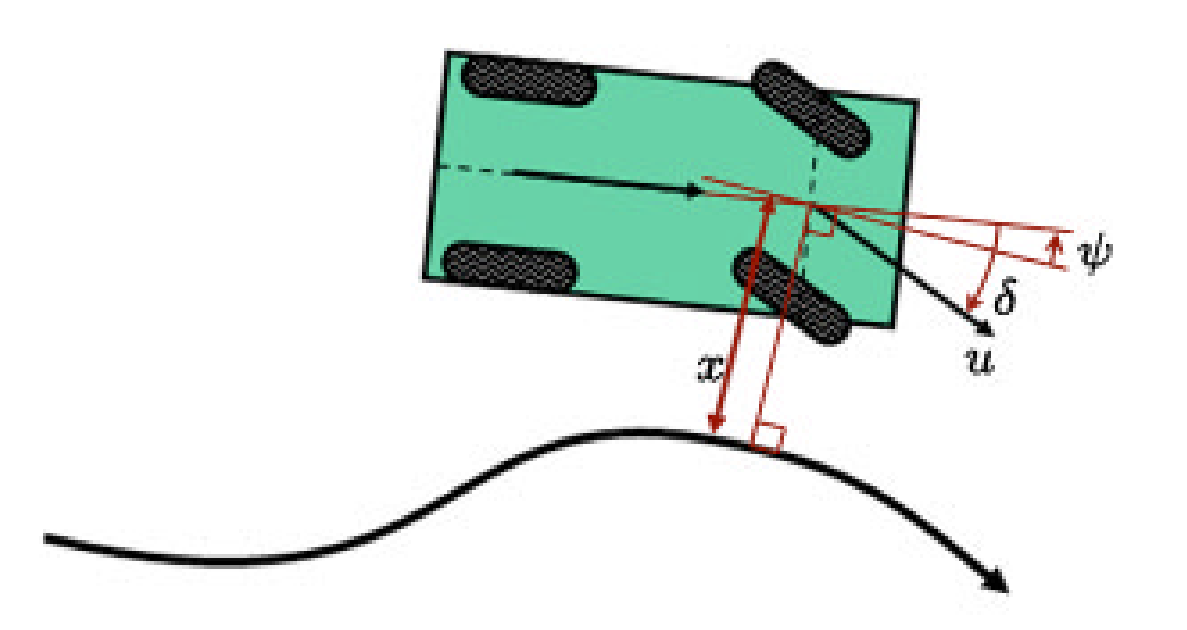
\includegraphics[width=.8\textwidth]{figures/stanley-control.png}
\caption{The geometrical relation between the trajectory and the car used by
Stanley controller algorithm. Taken from \cite{Thrun2006StanleyTR}.}
\label{figure:stanley-control}
\end{figure}

Nonlinear feedback function of cross-track error is given by Equation
\eqref{eq:stanley-control}.

\begin{equation}
    \delta(t) = \psi(t) + \arctan\frac{kx(t)}{u(t)}\ \textbf{,}
\label{eq:stanley-control}
\end{equation}

where $k$ is a gain parameter, $u(t)$ is the car speed, and $\psi(t)$ denotes
the orientation of the nearest trajectory segment relative to the car's
orientation. The intuition behind the controller is that as the cross-track
error $x(t)$ increases, the controller produces stronger steering angle
$\delta(t)$ towards the trajectory.  Likewise, as the speed $u(t)$ increases,
the controller avoids sudden strong maneuvers. Hoffmann et al. studies the
Stanley controller algorithm in greater detail in
\cite{Hoffmann2007AutonomousAT}.

In 2007, DARPA Urban Challenge took place. Montemerlo et al. \cite{cite1}
presents the competition details and the software architecture of Junior,
Stanford's another robot car and the second best car in the challenge. This
time rules were more complex including overtaking parking or moving vehicles,
precedence handling at intersections possibly with stop signs, merging into
fast moving traffic, left turns, parking and U-turns when the road is
completely blocked. Participants were provided with a road network description
file or RNDF which contained lane information, stop signs, parking lots, and
special checkpoints. In addition, the teams were also provided with a high
resolution aerial image of the race course so that they can further improve the
RNDF. In the competition, the vehicles were given multiple missions as a
sequence of checkpoints in the RNDF.

Like Stanley, Junior's software software architecture is made of sensor
interfaces, perception, navigation, and drive-by-wire interfaces at the core.
The design is again based on data processing endpoints communicating with
publish/subscribe pattern. Unlike Stanley, Junior's modules are far more
advanced.  Junior's perception module segments the environment data into moving
vehicles and static obstacles. Its navigation features a global path planner
based on dynamic programming to find an optimum path to the mission checkpoints
from the current location of the car. Moreover, the navigation module handles
different driving scenarios with different planning algorithms.

It performs free-form navigation in parking lots, at U-turns or whenever the
car gets stuck for extended period of time. The free-form planner is
specifically developed for Junior and named hybrid A* by the Stanford Racing
Team. Hybrid A* associates discrete search space of regular A* with a
continuous state by performing forward simulations with different steering
angles and computes a score based on the continuous state. The continuous state
is represented by x-y position of the car, heading direction, and the
direction, either forward or reverse. Whereas the path found by the regular A*
and Field D* algorithms cannot be executed due to their discrete nature, hybrid
A* can find executable paths that the nonholonomic constaints of the vehicle.
Hybrid A* uses dual admissible heuristics. One heuristic is nonholonomic
without obstacles, and the other is holonomic with obstacles. Once a solution
is found, it is smoothed for a better driving experience. Extensive study and
experiments show that hybrid A* produces near-optimal solutions
\cite{Dolgov2010PathPF, Petereit2012Application}. Figure
\ref{figure:hybridastar-comparison} demonstrates the difference between regular
A*, Field D*, and hybrid A* algorithms.

\begin{figure}[h]
\centering
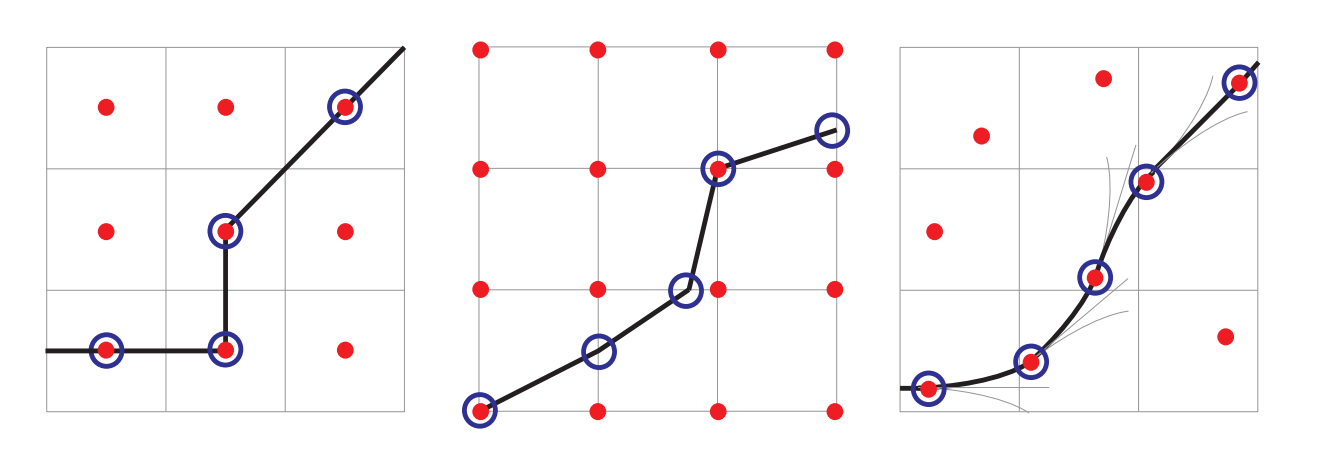
\includegraphics[width=.8\textwidth]{figures/hybridastar-comparison.png}
\caption{Left: Regular A* solutions passes through only the center of grids.
    Center: Field D* solutions can have arbitrary linear paths from cell to cell.
    Right: Hybrid A* associates a continuous state with each cell and compute a
score for the continuous state. Taken from \cite{Dolgov2010PathPF}.}
\label{figure:hybridastar-comparison}
\end{figure}

Junior uses a different planner for normal on-road navigation. It performs
internal simulations with different steering parameters. The internal
simulations generate candidate trajectories according a reference path. This
reference path is essentially the smoothed center of the lane obtained from
RNDF. The planner evaluates the candidate trajectories by a cost function and
finally selects the best trajectory. The cost function also regulates the lane
change or overtaking behavior of Junior. When the right lane is blocked, the
car chooses to shift left. When the overtaking is complete, it steers back to
the right lane as it would be more costly to occupy the left lane.

Driving behavior of Junior is governed by a hierarchical finite state machine.
The state machine decides on the U-turns, handles intersection precedence and
stop signs, prevents the car from getting stuck, switches to parking navigation
in a parking lot or chooses the true planner for the current scenario in
general.

Werling et al. \cite{cite14} reports that they generated optimal trajectories
in Frenet frame and tested it on Junior without obstacles. They also present
their obstacle avoidance experiments in simulation. In their method, they
suggest integrating trajectory generation with a behavioral layer that decides
on the high level as to whether the car should keep a constant velocity, follow
the car in front with a constant distance, merging into traffic or stoping at a
point. Figure \ref demonstrates a velocity keeping instance in this approach.

\begin{figure}[h]
\centering
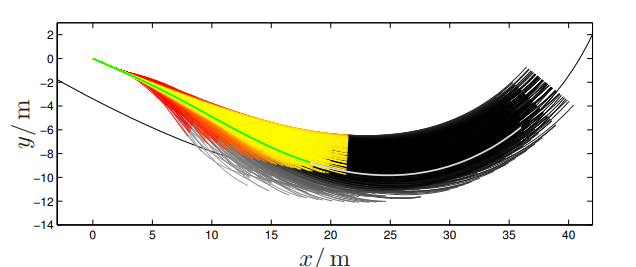
\includegraphics[width=.8\textwidth]{figures/frenet-velocity-keeping.png}
\caption{An exmaple optimal trajectory generated in Frenet frame in velocity
    keeping mode. Colors from red to yellow represent increasing lateral cost.
    Colors from grey to black represent increasing longitudinal cost. Green and
    light grey colors represent the optimal trajectory, which leads the car to
    the reference line and desired speed. Taken from \cite{cite14}.}
\label{figure:autoware}
\end{figure}

Yoneda et al. \cite{cite15} further extends the method in \cite{cite14}
introducing an additional adjust mode while switching from velocity keeping
mode or cruise mode to distance keeping in an affort to eliminate strong
acceleration and deceleration during the mode switching in the quest of a more
natural driving experience.

Fast forward to the present day, Autoware \cite{Kato2018Autoware0B}, being one
of the modern open source self-driving car platform is based on ROS
\cite{cite3}. ROS is a commonly used, extendible, component based, higly
modular middleware framework with many reusable packages and visualization
tools that dramatically accelerated today's robot development and prototyping
processes.  Unsurprisingly, publish/subscribe mechanism is at the core of ROS
communication patterns. Autoware implements perception, decision-making,
planning and path tracking capabilities. Figure \ref{figure:autoware}
illustrates the the Autoware architecture at a high level.

\begin{figure}[h]
\centering
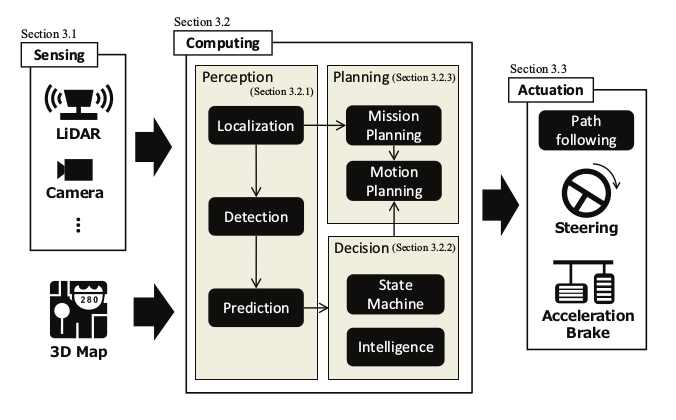
\includegraphics[width=.8\textwidth]{figures/autoware.png}
\caption{Autoware high level architecture and data flow. Taken from
    \cite{Kato2018Autoware0B}.}
\label{figure:autoware}
\end{figure}

Perception capabilities are made of localization, detection, and prediction
modules. For the localization, Autoware relies on high definition 3D maps. It
localizes itself appling scan matching between the 3D map and LiDAR scans.
Therefore, a 3D map of the environment should be created beforehand using SLAM
technologies, in which scan matching is applied against previous LiDAR scans
instead of a 3D map such that a transformation between the LiDAR scans are
obtained and a cumulative point cloud is continually updated. Other perception
modules are also rely on the localization. For example, the car is localized in
the 3D map, it projects 3D map fatures into the front view camera images to
define a ROI for traffic light detection and classification in order to
eliminate full image search on every image frame. The detection module supports
both deep learning and traditional image processing and machine learning
techniques. It features YOLO2 \cite{Redmon2016YOLO9000BF} and SSD
\cite{Liu2016SSDSS} models for detecting objects in the traffic such as traffic
signals, pedestrians, and other vehicles. In the prediction module, Autoware
associates detected objects with time, so that it estimates trajectories for
the moving objects which are then used in the planning modules. Based on the
perception modules, Autoware makes decisions in response to the environmental
changes. The decision-making scheme is captured in a finite state machine
similar to Junior.

Autoware features two set of planners, a mission planner and motion planners.
The mission planner is responsible for a rough global path from the current
location to the destination in the map. Motion planners, on the other hand,
generates local trajectories taking the global plan as a reference. In
unstructured environments such as parking lots, hybrid A* is used similar to
Junior. For well-structured environment scenarios such as navigating on the
lanes, state lattice based algorithms are preferred. Pivtoraiko et al.
\cite{Pivtoraiko2009DifferentiallyCM} introduces space lattice based planning.
The state lattice is made of motion primitives of a specific car. The motion
primitives are generated offline by a precise trajectory generator respecting
the mobility model of the vehicle such as steering limits and wheelbase. Then,
the lattice search space could be search by D* algorithms for optimal
trajectories. This method also successfully used in DARPA Urban Challenge by
the winner vehicle, Carnegie Mellon University's Tartan Racing for navigating
in unstructural environments \cite{Urmson2007TartanRA}. Figure
\ref{figure:state-lattice} illustrates a state lattice. McNaughton et al.
\cite{McNaughton2011MotionPF} later extended this approach and applied it to
structural environments.

\begin{figure}[h]
\centering
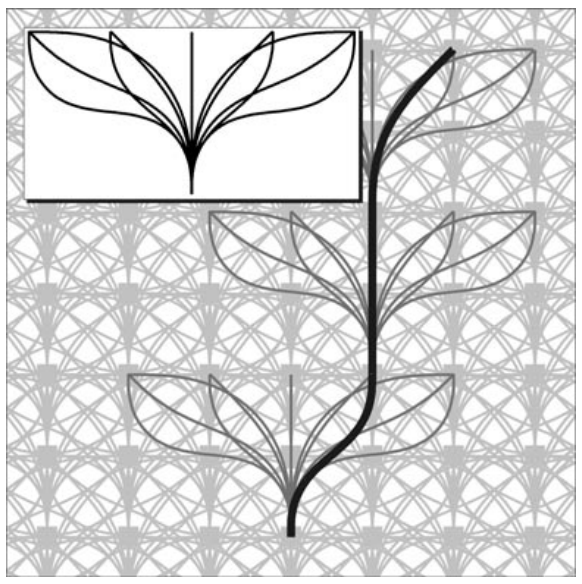
\includegraphics[width=.8\textwidth]{figures/state-lattice.png}
\caption{An example state lattice without reverse motions. Taken from
\cite{Pivtoraiko2009DifferentiallyCM}.}
\label{figure:state-lattice}
\end{figure}

Autoware uses pure pursuit controller to generate low level steering commands
to execute the given trajectory from the motion planners. Kim et al.
\cite{cite18} studies the controller with its geometrical derivation and also
gives some useful pointers on tuning.

Backed by Baidu, Apollo is another open source autonomous driving platform with
its giant dataset \cite{Huang2018TheAD}. Similar to other other decompositioned
architectures, Apollo is also made of localization, perception, prediction,
routing, motion planner, and vehicle control components as shown in Figure
\ref{figure:apollo}. Like Autoware, Apollo also relies on high definition 3D
maps for location and perception \cite{Fan2018BaiduAE}.

\begin{figure}[h]
\centering
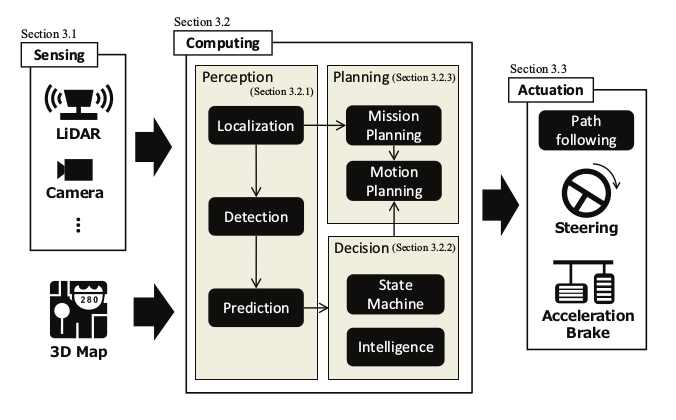
\includegraphics[width=.8\textwidth]{figures/autoware.png}
\caption{Apollo high level architecture and data flow. Taken from
    \cite{Fan2018BaiduAE}.}
\label{figure:autoware}
\end{figure}

The routing component finds a global plan from the current location
to a destination in the map like previous architectures; however, Apollo's
lane-based motion planner is quite different. Apollo does not directly use
this global plan as a reference path for trajectory generation, but rather it
generates multiple lane level reference lines from it taking traffic
regulations (e.g., traffic signs, signals and lane markings) and safety
measures into account.  During lane level motion planning, Frenet frames are
constructed based on the given reference lines.  Lane level path and speed
optimizers generate the optimal trajectories in Frenet frame for each lane.
Finally, a trajectory decider chooses the best trajectory for the maneuver
given the cost of each trajectory, car status, traffic regulations.  This
approach allows for dealing with different traffic regulations that apply for
different lanes of the same road \cite{Fan2018BaiduAE}.

A different approach to autonomous cars is to learn a mapping from input images
to steering angle and speed commands in an end-to-end manner. Bojarski et al.
\cite{Bojarski2016EndTE} were the first to apply this method to a real-sized
car with the modern deep learning advancement. They collected 72 hours data
with different cars in different weather and lighting conditions from various
places. For the data acqusition, they installed three cameras on the car behind
the windshild and recorded timestamped videos from the left, right and center
cameras along with the steering commands controlled by a human driver. During
training, they agumented the dataset by random shifting and rotating the images
and adjusting the recorded commands accordingly. The trained model then
successfully steered the car by using the images only from the central camera.
Figure \ref{figure:end-to-end-network} demonstrates the training and testing
steps of this approach.

\begin{figure}[h]
  \centering
  \begin{subfigure}[b]{0.4\linewidth}
      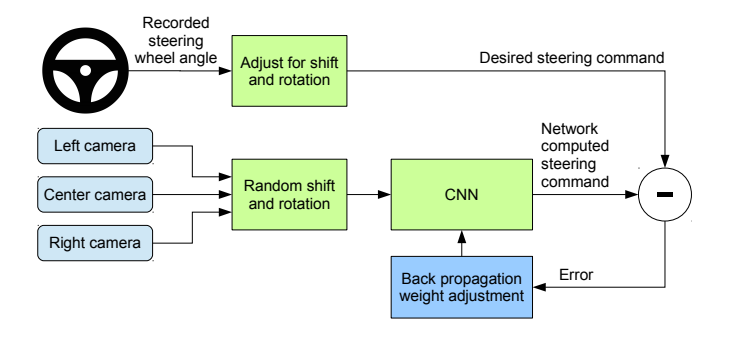
\includegraphics[width=\linewidth]{figures/end-to-end-training.png}
    \caption{}
  \end{subfigure}
  \begin{subfigure}[b]{0.4\linewidth}
      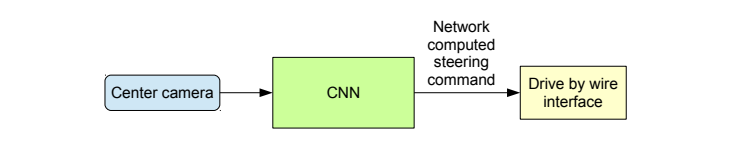
\includegraphics[width=\linewidth]{figures/end-to-end-inference.png}
    \caption{}
  \end{subfigure}
  \caption{(a) End-to-end training scheme. (b) Steering command inference from
  raw camera images. Taken from \cite{Bojarski2016EndTE}.}
  \label{figure:end-to-end-network}
\end{figure}

Bechtel et al. \cite{Bechtel2017DeepPicarAL} relicated the work
\cite{Bojarski2016EndTE} with a small-scale, low-cost platform using a web
camera and Raspberry Pi 3 for inference. They conducted successful experiments
in a specially built test course for the RC car.

Do et al. \cite{Do2018RealTimeSC} also implemented a similar approach in
another RC car platform using Pi camera and Raspberry Pi 3 for inference.
Instead of learning steering angles in a regression model, they learned a
steering angle probability for discretized steering angle space. In addition to
basic lane following, they also learned to turn left or right when the
corresponding traffic sign is encountered. The traffic sign diameter was 15 cm
in their experiments.

There are several traffic scene segmentation segmentation datasets available.
Currently, the largest and the most comprehensive is ApolloSpace
\cite{Huang2018TheAD}. It is followed by Cityscapes \cite{Cordts2016TheCD},
KITTI \cite{Geiger2012AreWR}, and Mapillary Vistas \cite{Neuhold2017TheMV}
datasets. Because these datasets are created for real-sized cars on the real
roads, they were not much useful for us, so we had to create our own
segmentation dataset. The existing traffic sign and signal classification
datasets \cite{cite11, cite12, Shakhuro2016RussianTS,
Serna2018ClassificationOT, MaldonadoBascn2007RoadSignDA}, on the other hand,
was useful to train an initial classifier as they are mostly independent of the
scene and car size.

Sakai et al. \cite{cite18} presents a collection of various autonomous
navigation algorithms implemented in Python Programming Language in their basic
forms. The collection includes aforementioned hybrid A*, frenet optimal
trajectory planner, state lattice planner, stanley controller, and pure pursuit
controller algorithms.

Unlike Stanley, Junior, Autoware and Apollo, we don't have a detailed map of
the driving course. As a result, our best option is to follow the lanes unless
a traffic sign or another conditions mandate otherwise. For the same reason, we
have to create our reference paths for our local trajectory generation either
from the online detected lane centers or according to the traffic regulations.
Meyer et al. \cite{cite9} studies semantic lane segmentation for mapless
driving, which bears similaries to our lane detection approach.  Autohors
motivation is the fact that as the high definition maps quickly gets out of
date due to constructions an autonomous car should also be able to perform
basic navigation tasks without a precise map, but possibly with a course map,
specifically for intersections. They start with creating their own dataset by
extending Cityscape \cite{Cordts2016TheCD}. Their approach is to annotate the
road surface as ego lane, parallel lane, and opposite lane and learn these
regions with a semantic segmentation model.

Stanley controller algorithm is weak to discontinuities along the trajectory as
it directly drives towards the closest point on the trajectory. Stanley and
Junior guarantees a smooth trajectory by smoothing already known center
reference lines or post processing the output of hybrid A*. We cannot guarantee
a smooth path as we use discontinuous predefined path in response to traffic
signs and signals or due to instantaneous segmentation errors in the lane
detection.  Conversely, as pure pursuit controller drives along an arc it is
less likely to be affected by discontinueties.
